\documentclass[a4paper,11pt,oneside,showtrims]{alpenthesis}
\usepackage{lipsum}
\hextrue
\paperfalse

%% ================================================================= SET TITLE %
\title{My Thesis}
\author{Raphael Frey \\[1ex]\href{https://github.com/alpenwasser/}
                                 {\nolinkurl{https://github.com/alpenwasser/}}}

\chapterstyle{alpenthesis}
%% ============================================================== END PREAMBLE %
\begin{document}
%% ============================================================= BEGIN CONTENT %
\begin{hextitlingpage}
    \tikzset{external/export next=false}%
    \begin{tikzpicture}[remember picture,overlay]
        \node[anchor=north east,yshift=-5mm,xshift=-10mm]
            at (current page.north east)
            {
\includegraphics[height=10mm]{logo-top.pdf}};
    \end{tikzpicture}
    \tikzset{external/export next=false}%
    \begin{tikzpicture}[remember picture,overlay]
        \node[anchor=south east,yshift=+5mm,xshift=-10mm]
            at (current page.south east)
            {
\includegraphics[height=16mm]{logo-bottom.pdf}};
    \end{tikzpicture}
    \flushright\sffamily

    \vspace{3ex}
    \Huge\bfseries{A Mostly Appropriate Title}\\[1ex]
    \Large\mdseries{Thesis}\\[3ex]

    \normalsize\mdseries

    alpenwasser\\
    team partner\\[3ex]

    Supervisor\\
    Expert\\

    \vfill

    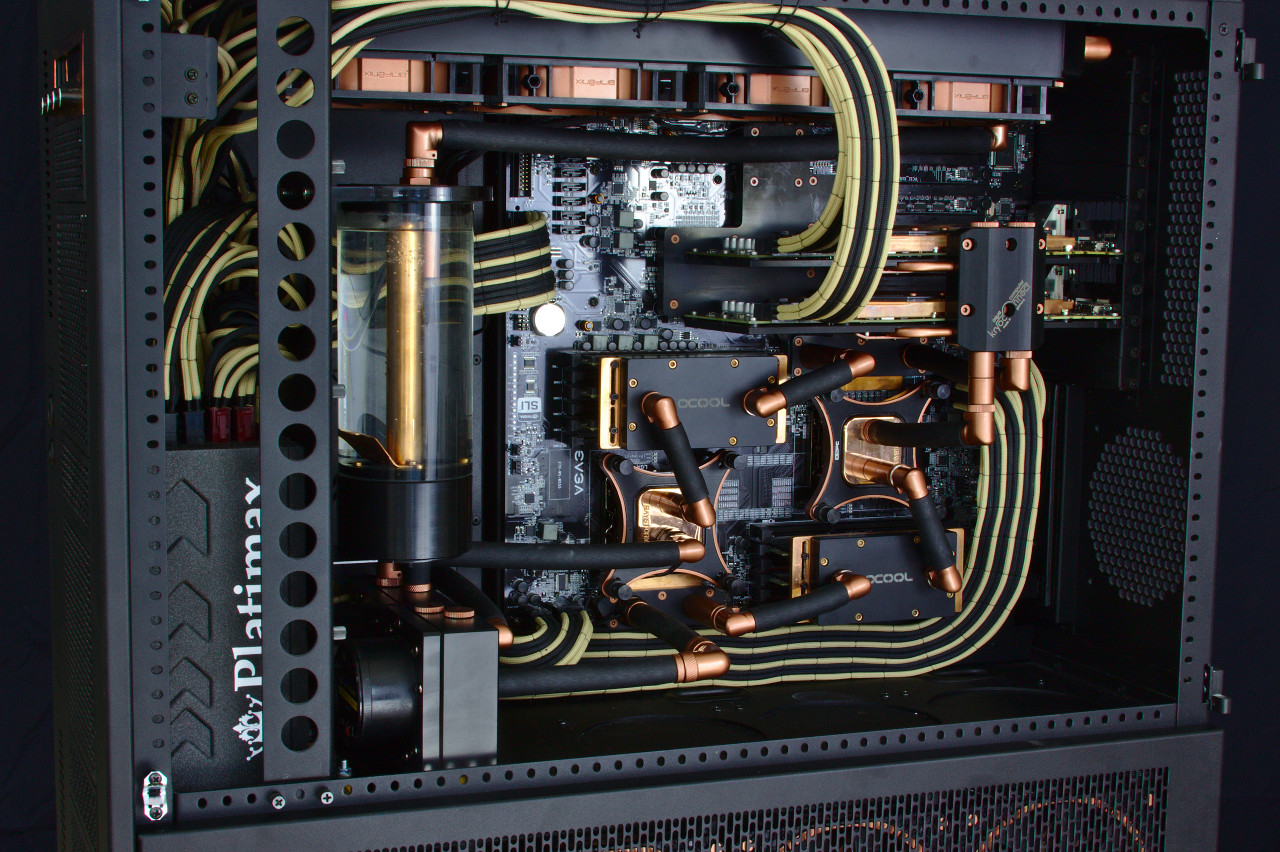
\includegraphics[width=120mm]{titlepic.jpg}

    \vfill

    \today\\
    Version 1.0.0
\end{hextitlingpage}
\frontmatter
\tableofcontents*

\mainmatter
\chapter{Showcase}

\lipsum[1-2]
This chapter presents a show case of the \athes\ document class configuration.
This includes fonts, colors, tables, figures, headings etc.

\section{Fonts}

The default  font family  is \pacname{kpfonts}  in 11\,pt  for both  roman and
\textsf{sans serif  style}, and  \pacname{DejaVuSansMono} \texttt{is  used for
for monospace text}, scaled at a factor of  0.8125 so that the x height is the
same as the x height of the default roman font.

\section{Floats and Captions}

We put  this in  a \verb|\subsection|  and have some  padding text  around the
floats courtesy of the \pacname{lipsum} package.

\begin{table}
    \centering
    \caption{tabular inside float}
    \label{tab:float}
    \begin{tabular}{lll}
        \toprule
        \scshape Header 1 & \scshape Header 2 & \scshape Header 3 \\
        \midrule
        Content           & Content           & Content           \\
        Content           & Content           & Content           \\
        Content           & Content           & Content           \\
        Content           & Content           & Content           \\
        \bottomrule
    \end{tabular}
\end{table}

\lipsum[3]

\begin{center}
    \tabcaption{Tabular outside of float}
    \label{tab:outside}
    \begin{tabular}{lll}
        \toprule
        \scshape Header 1 & \scshape Header 2 & \scshape Header 3 \\
        \midrule
        Content           & Content           & Content           \\
        Content           & Content           & Content           \\
        Content           & Content           & Content           \\
        Content           & Content           & Content           \\
        \bottomrule
    \end{tabular}
\end{center}

This sentence refers to Table~\ref{tab:outside}.

This is a citation \cite{testitem}.

\href{https://hyperlink.com}{This is a hyperlink hiding behind text.}

\href{https://hyperlink.com}{\nolinkurl{https://hyperlink.com}}

\section{Sectional Headings}

This section illustrates the  style of \verb|\section|, \verb|\subsection| and
\verb|\subsubsection|.

\subsection{A Subsection}

\lipsum[1]

\subsubsection{A subsubsection}

\lipsum[2]

\appendix\chapterstyle{alpenappendix}
\chapter{An Appendix Chapter}
\lipsum[1-3]

\chapter{Another Appendix Chapter}

\tikzset{external/export next=false}%
\begin{tcblisting}{%
        title=This Is a Code Listing,
        minted language=tex,
        listing side text,
        }
    \begin{tabular}{ll}
        a & a \\
        a & a \\
    \end{tabular}
\end{tcblisting}

\tikzset{external/export next=false}%
\begin{tcolorbox}[title=test]
    \lipsum[2]
\end{tcolorbox}

\tikzset{external/export next=false}%
\begin{tcolorbox}
    \lipsum[2]
\end{tcolorbox}

\chapter{Another Appendix Chapter}
\lipsum[4-6]

\chapter{Another Appendix Chapter}
\lipsum[4-6]

\chapter{Another Appendix Chapter}
\lipsum[4-6]

\backmatter
\chapter{A Backmatter Chapter}
\lipsum[7-9]

\begin{thebibliography}{1}
    \bibitem{testitem}
        An Author, ``A Title``, 1979.
\end{thebibliography}
\end{document}
